\documentclass[10pt,letterpaper]{article} % {{{
\usepackage[top=0.85in,left=2.75in,footskip=0.75in]{geometry}
\usepackage{amsmath,amssymb}
% Use adjustwidth environment to exceed column width (see example table in text)
\usepackage{changepage}

% textcomp cpackage and marvosym package for additional characters
\usepackage{textcomp,marvosym}
\usepackage{subcaption}


\usepackage[T1]{fontenc}
\usepackage{lmodern}
% cite package, to clean up citations in the main text. Do not remove.
\usepackage{cite}

% Use nameref to cite supporting information files (see Supporting Information section for more info)
\usepackage{nameref,hyperref}

% line numbers
\usepackage[mathlines]{lineno}  \linenumbers \setlength\linenumbersep{3pt}

% ligatures disabled
\usepackage[nopatch=eqnum]{microtype}
\DisableLigatures[f]{encoding = *, family = * }

% color can be used to apply background shading to table cells only
\usepackage[table]{xcolor}

% array package and thick rules for tables
\usepackage{array}
\usepackage{caption}
\captionsetup[figure]{labelfont={bf},labelformat={default},labelsep=period,name={Fig}}


% create "+" rule type for thick vertical lines
\newcolumntype{+}{!{\vrule width 2pt}}

% create \thickcline for thick horizontal lines of variable length
\newlength\savedwidth
\newcommand\thickcline[1]{%
  \noalign{\global\savedwidth\arrayrulewidth\global\arrayrulewidth 2pt}%
  \cline{#1}%
  \noalign{\vskip\arrayrulewidth}%
  \noalign{\global\arrayrulewidth\savedwidth}%
}

% \thickhline command for thick horizontal lines that span the table
\newcommand\thickhline{\noalign{\global\savedwidth\arrayrulewidth\global\arrayrulewidth 2pt}%
\hline
\noalign{\global\arrayrulewidth\savedwidth}}


% Remove comment for double spacing
%\usepackage{setspace} 
%\doublespacing

% Text layout
\raggedright
\setlength{\parindent}{0.5cm}
\textwidth 5.25in 
\textheight 8.75in

% Bold the 'Figure #' in the caption and separate it from the title/caption with a period
% Captions will be left justified
\usepackage[aboveskip=1pt,labelfont=bf,labelsep=period,justification=raggedright,singlelinecheck=off]{caption}
\renewcommand{\figurename}{Fig}
\renewcommand{\succ}{\textrm{succ}}

\newcommand{\fref}[1]{Fig~\ref{#1}}
\newcommand{\eref}[1]{Eq~(\ref{#1})}
% Use the PLoS provided BiBTeX style
\bibliographystyle{plos2015}

% Remove brackets from numbering in List of References
\makeatletter
\renewcommand{\@biblabel}[1]{\quad#1.}
\makeatother



% Header and Footer with logo
\usepackage{lastpage,fancyhdr,graphicx}
\usepackage{epstopdf}



\usepackage[english]{babel}
\usepackage{graphicx,helvet}
\usepackage{color}
\usepackage{url}
\usepackage{amssymb}
\usepackage[utf8]{inputenc}
\usepackage{hyperref}
% \usepackage[inline]{showlabels}
\usepackage{bbm,bm}
\usepackage{soul}
\usepackage{amsfonts}

\usepackage{tikz}
\usetikzlibrary{arrows}
\usetikzlibrary{quantikz}

\usepackage[draft,inline,nomargin]{fixme} \fxsetup{theme=color}
\FXRegisterAuthor{cp}{acp}{\color{blue}CP}
\FXRegisterAuthor{tb}{ttb}{\color{green}TB}
\FXRegisterAuthor{rev}{rrv}{\color{red}REV}



%\pagestyle{myheadings}
\pagestyle{fancy}
\fancyhf{}
%\setlength{\headheight}{27.023pt}
\rfoot{\thepage/\pageref{LastPage}}
\renewcommand{\headrulewidth}{0pt}
\renewcommand{\footrule}{\hrule height 2pt \vspace{2mm}}
\fancyheadoffset[L]{2.25in}
\fancyfootoffset[L]{2.25in}
\lfoot{\today}

%% Include all macros below

\newcommand{\lorem}{{\bf LOREM}}
\newcommand{\ipsum}{{\bf IPSUM}}
\DeclareMathOperator{\tr}{tr}
\newtheorem{definition}{Definition}
\newtheorem{theorem}{Theorem}

%% END MACROS SECTION

% }}}
\begin{document}
% Titulo, afiliacion, abstract  {{{
\vspace*{0.2in}

\begin{flushleft}
{\Large
\textbf\newline{Quantum simulation of Pauli channels and dynamical maps: algorithm and implementation } % Please use "sentence case" for title and headings (capitalize only the first word in a title (or heading), the first word in a subtitle (or subheading), and any proper nouns).
}
\newline
% Insert author names, affiliations and corresponding author email (do not include titles, positions, or degrees).
\\
Tomás Basile\textsuperscript{1,2\Yinyang},
Carlos Pineda\textsuperscript{2*\Yinyang},
\\
\bigskip
\textbf{1} Facultad de Ciencias. Universidad Nacional Autónoma de México, Ciudad de México, Mexico
\\
\textbf{2} Instituto de Física, Universidad Nacional Autónoma de México, Ciudad de México, México
\\
\bigskip

% Insert additional author notes using the symbols described below. Insert symbol callouts after author names as necessary.
% 
% Remove or comment out the author notes below if they aren't used.
%
% Primary Equal Contribution Note
\Yinyang These authors contributed equally to this work.

% Additional Equal Contribution Note
% Also use this double-dagger symbol for special authorship notes, such as senior authorship.
% \ddag These authors also contributed equally to this work.

% Current address notes
% \textcurrency Current Address: Dept/Program/Center, Institution Name, City, State, Country % change symbol to "\textcurrency a" if more than one current address note
% \textcurrency b Insert second current address 
% \textcurrency c Insert third current address

% Deceased author note
% \dag Deceased

% Group/Consortium Author Note
% \textpilcrow Membership list can be found in the Acknowledgments section.

% Use the asterisk to denote corresponding authorship and provide email address in note below.
* carlospgmat03@gmail.com

\end{flushleft}
% Please keep the abstract below 300 words
\section*{Abstract}
Pauli channels are fundamental in the context of quantum computing as they
model the simplest kind of noise in quantum devices.  We propose a quantum
algorithm for simulating
Pauli channels 
and extend it to encompass Pauli dynamical maps 
(parametrized Pauli channels).
A parametrized quantum circuit is employed to accommodate for dynamical maps. 
We also establish the mathematical conditions for an
$N$-qubit transformation to be achievable using a parametrized circuit where
only one single-qubit operation depends on the parameter. 
The implementation of the proposed circuit is demonstrated using IBM's quantum computers 
for the case of one qubit, and the fidelity of this implementation is reported. 
% Please keep the Author Summary between 150 and 200 words
% Use first person. PLOS ONE authors please skip this step. 
% Author Summary not valid for PLOS ONE submissions.   
%\section*{Author summary}


% Use "Eq" instead of "Equation" for equation citations.


% }}}
\section{Introduction} % {{{


% Citar a estos manes de alguna manera y pedir que nos citen;
% https://mail.google.com/mail/u/0/#inbox/FMfcgzGtwgbtTGtlXkBtrCGQRxjRZrph

Since their inception, quantum computers were proposed as powerful tools for
the simulation of quantum systems~\cite{feynman1982simulating}.  Being open
quantum systems of fundamental~\cite{Zur91,RevModPhys.76.1267} and
practical~\cite{breuer2007theory} interest, there has been efforts towards the
simulation of the evolution of open quantum systems~\cite{Garcia, Wang,Weimer}
and specifically for quantum channels~\cite{He-Lu,Xin,Wei,Zanetti}, 
which can be used to study and model decoherence.
Such quantum algorithms can be represented using what is known as a quantum
circuit~\cite{chuangbook}, which we will study in section \ref{sec: Circuit for a Pauli Channel}.

Such systems have been simulated because of their many applications, such as
studying the emergence of multipartite entanglement~\cite{Andrea,Andrea_AD},
studying dissipative processes~\cite{Barreiro} and modeling non-Markovian
dynamics~\cite{Marsden}.  Among quantum systems, the simplest case is that of a
qubit~\cite{chuangbook}, and within them, the simplest class of channels that
produce decoherence are Pauli channels~\cite{geometry,Zbigniew,Davalos}.
Indeed, they serve as effective models for the noise affecting quantum
devices~\cite{Flammia}.

In this article we propose a quantum algorithm for simulating Pauli channels
and implement it on one of IBM's quantum computers.  The algorithm proposed is
straightforward and can be used for any Pauli channel by only changing a couple
of parameters in the operations it performs.  To represent the algorithm, we
use a quantum circuit, which is a common way of representing algorithms
intended for quantum computers.~\cite{chuangbook}.  Furthermore, we will also
simulate Pauli dynamical maps, which are continuous parametrized curves of
Pauli channels.  These maps can be used to model a continuous change of a qubit
instead of only discrete jumps.  The generality of the algorithm proposed for
Pauli channels will be very useful in this part, since then using for dynamical
maps will come very naturally.  Implementing these maps will lead us to study
quantum algorithms  with free parameters, something that is common in areas
such as quantum machine learning~\cite{Benedetti}.  This can be done using
parametrized quantum circuits, which consist of quantum circuits in which one
or more operations depend on a free parameter. 


We start by providing the definition of quantum channels, the general framework
used here, and multi-qubit Pauli channels in section \ref{sec: Pauli Channels}.
Our first objective is to present a general and straightforward quantum algorithm capable of simulating
Pauli channels on quantum computers; we do this in section \ref{sec: Circuit
for a Pauli Channel}, where we also demonstrate its implementation using IBM's
quantum computers for several single and two-qubit Pauli channels.
Expanding beyond Pauli channels, we introduce the concept of Pauli
dynamical maps, defined as a continuous parametrization of multi-qubit Pauli
channels. In fact, in order  to implement them, we study parametrized quantum
circuits in chapter \ref{sec: 1PR Circuits}. Furthermore, we contribute to the body of work
related to parametrized quantum circuits by establishing a theorem, which  sets
the mathematical conditions for the transformations that can be done using a
parametrized circuit with the restriction that only a controlled single-qubit
rotation in the circuit may depend on the parameter.  Finally, in section
\ref{sec: 1PR circuit for a Pauli map}, we conclude analyzing the Pauli
dynamical maps that fulfill the conditions of theorem \ref{theorem2}. 


%
%We start the article by providing the definition of quantum channels, the
%general framework used here, and multi-qubit Pauli channels in section
%\ref{sec: Pauli Channels}.  Then, since our main objective is to obtain a
%parametrized circuit for Pauli dynamical maps, we will first need a circuit
%that can implement any Pauli channel by only changing some parameters in the
%quantum gates and without changing the design of the circuit itself.
%Therefore, in section\ref{sec: Circuit for a Pauli Channel} we present such a
%circuit and we also show its implementation using IBM's quantum computers for
%the particular case of single-qubit Pauli channels and some two-qubit ones.  In
%section \ref{sec: 1PR Circuits}, we adapt the algorithm to dynamical maps.
%Then we aim to simplify the algorithm so that it only contains one parametrized
%single-qubit rotation, and in the process we contribute to the work in
%parametrized quantum circuits by establishing   in \ref{theorem2} which general
%quantum transformations can be implemented this way.  Finally, in section
%\ref{sec: 1PR circuit for a Pauli map}, we conclude analyzing the Pauli
%dynamical maps that fulfill the conditions of theorem \ref{theorem2}.  
 

% \revnote{I fail to see the point here - the logic of the paper is: % {{{
% 1."open quantum systems can be modeled through a class of channels representing
% he various types of decoherence. 2. Quantum circuits are a convenient
% gate-based formalism that is well understood and has an extensive body of work,
% and experimentally accessible.  3. We map (generalised) Pauli channels onto
% quantum circuits, as a way to simulate them. \\
% What I am missing is what do we learn by doing it which can't be learned by
% actually performing the Pauli channel onto a quantum system? For example,
% applying well controlled sx, sy, sz operations and their coherent parametric
% combination using a photonic polarisation or path encoding is experimentally
% trivial. Why would I need to decompose (not even effectively for any channel)
% the Pauli channels to match a gate based description? Which class of problems
% can we simulate that cannot be simulated otherwise? Is there any advantage (for
% example in speed up, resources like ancillas required, resistance to unwanted
% noise etc..?)\\
% Intuitively, it seems incredibly harder resource wise to create the sum
% $b|gamma\rangle$ superposition state needed for the ancilla, just for the sake
% of having it into a "quantum circuit" perspective.} % }}}



% }}}
\section{Pauli channels and dynamical maps}  \label{sec: Pauli Channels} % {{{

% Intro  {{{

In this section  we introduce the concept of quantum channels, focusing on a
specific type called Pauli channels.  Furthermore, we define Pauli dynamical
maps, which are curves of Pauli channels parametrized by a variable.
% }}}
\subsection{Quantum channels} \label{subsec: Quantum Channels} % {{{


In quantum mechanics, a closed system's state is represented by a vector in a
Hilbert space $\mathcal{H}$.  The state's evolution is unitary and given by
Schrodinger's equation~\cite{Rieffel}.  However, in real-world situations,
quantum systems are usually open, which means that they interact with their
environment~\cite{breuer2007theory}.  For instance, the system's state may become
entangled with the environment, leading to a loss of information about the
system's state over time.

To describe open systems, instead of state vectors, we use matrices $\rho$ that
act on $\mathcal{H}$.  These matrices are called density matrices, and they
include information about the system's interaction with its environment.  For a
density matrix $\rho$ to be physically valid, it must satisfy two conditions:
$\tr(\rho) = 1$ and it must be positive semi-definite, which is denoted as
$\rho \geq 0$~\cite{chuangbook}.


Knowing this, we can now define quantum channels.  Quantum channels are
operators $\mathcal{E}$ that can describe the evolution of open quantum
systems, such that $\rho \rightarrow \mathcal{E}(\rho)$.  Quantum channels are
the most general linear operations that a quantum system can undergo
independently of its past~\cite{zimansbook,cirac}.  These channels are
constructed based on three fundamental properties: linearity, trace
preservation, and complete positivity.

Linearity ensures that a quantum channel $\mathcal{E}$ maps any ensemble of
density matrices into the corresponding ensemble of their evolution.  The trace
preserving property is given by $\tr (\mathcal{E}[\rho]) = \tr (\rho) = 1$ and
guarantees that the quantum channel does not change the condition that
$\tr(\rho) = 1$.  Finally, the channel should also preserve the condition $\rho
\geq 0$, and a map that does this is called a positive map.  However,
positivity of $\mathcal{E}$ is not enough, and we actually require the more
restrictive condition of complete positivity.  Complete positivity means that
$\mathcal{E} \otimes \mathbb{I}_n$ is positive for any positive integer $n$
(where $\mathbb{I}_n$ is the $n\times n$ identity matrix).  This ensures that
even if the main system is entangled with another system, applying
$\mathcal{E}$ to the main system while doing nothing to the other one
still results in  a positive semidefinite state for the main
system~\cite{chuangbook}. 

Given a quantum channel $\mathcal{E}$, the condition of trace preservation is
straightforward to verify but complete positivity is not as simple.  To test
complete positivity of a quantum channel, Jamiołkowski and
Choi~\cite{choi,jamil} developed a simple algorithm that exploits the
isomorphism between a channel $\mathcal{E}$ and the state $\mathcal{D} =
(\mathbb{I} \otimes \mathcal{E}) [|\Omega \rangle \langle  \Omega|]$, where
$|\Omega\rangle = 1/\text{dim}(\mathcal{H}) \sum_{i}^{\text{dim}(\mathcal{H})}
|i \rangle |i \rangle$ is a maximally entangled state between the original
system and an ancilla.  Remarkably, the map $\mathcal{E}$ is completely
positive if and only if $\mathcal{D}$ (also known as the Choi or dynamical
matrix of $\mathcal{E}$) is positive semidefinite.

% }}}
\subsection{Pauli channels}  \label{subsec: Pauli Channels} % {{{

We have discussed the main features of quantum channels and 
now we turn our attention to a specific 
type of channels for $N$-qubit systems called Pauli channels.
First we will define these channels for single-qubit systems,
whose most general density matrix can be written as~\cite{chuangbook}:
\begin{equation}
\label{eq: Density Matrix}
\rho = \dfrac{1}{2} \sum_{\alpha=0}^{3} r_{\alpha} \sigma_{\alpha},
\end{equation}
with $\sigma_0 = \mathbb{I}$, and $\sigma_{1,2,3}$ the usual Pauli matrices.
The condition $\tr(\rho) = 1$ requires that $r_0 = 1$ while $\rho \geq 0$ 
implies that the remaining $r_{1,2,3}$ form
a vector $\vec{r}= (r_1,r_2,r_3)$ inside a unit sphere known as the Bloch sphere~\cite{Marinescu}.
That is, every possible density matrix for a one-qubit
system is uniquely associated with a point in a unit sphere. 

Given a one-qubit system described by $\rho$, 
a Pauli channel is defined as an operation that with probability $k_{\gamma}$
applies the Pauli matrix $\sigma_{\gamma}$ to
the system, for $\gamma = 0,1,2,3$~\cite{geometry}.
Mathematically, the Pauli channel is written in the following way:
\begin{eqnarray}
\label{eq: Pauli channel 1 qbit}
\mathcal{E}(\rho) = \sum_{\gamma=0}^3 k_{\gamma} \sigma_{\gamma} \rho \sigma_{\gamma},
\end{eqnarray} 
where the probabilities $k_{\gamma}$ of applying $\sigma_{\gamma}$
are non-negative real numbers such that 
$\sum_{\gamma} k_{\gamma} = 1$ (these conditions also ensure that the channel is 
trace preserving and completely positive).

Pauli channels are some of the 
most fundamental noise models in quantum information science~\cite{Terhal}. 
Some notable examples of Pauli channels are the following:
\begin{itemize}
\item \textbf{Bit Flip Channel:} This is a channel that with probability $1-p$ leaves the qubit as it is 
and with probability $p$ applies the $\sigma_1$ matrix 
(which flips the basis states $|0\rangle$ and $|1\rangle$ of the qubit), and
so it is given by:
\begin{align*}
\mathcal{E}(\rho) = (1-p) \rho + p \sigma_1 \rho \sigma_1.
\end{align*}
Analogous channels exist using $\sigma_3$ (called the bit flip channel,
which has a probability $p$ of adding a relative phase $\pi$ to the state) or 
using $\sigma_2$ (called the phase flip channel, 
which has a probability $p$ of 
flipping the base states and also add a relative phase $\pi$).
\item \textbf{Depolarizing channel:} 
This channel has a probability $1-p$
of doing nothing to the qubit and a probability $p$ of converting it into the maximally mixed state $\dfrac{1}{2} \mathbb{I}$
and it can be written as:
\begin{equation}
\mathcal{E}(\rho) = (1-p)\rho + p \dfrac{1}{2} \mathbb{I} = \left(1 - \dfrac{3p}{4} \right) \sigma + \dfrac{p}{4} \sigma_1 \rho \sigma_1 + \dfrac{p}{4} \sigma_2 \rho \sigma_2+ \dfrac{p}{4} \sigma_3 \rho \sigma_3.
\end{equation} 
\end{itemize}

We can also see how an arbitrary Pauli channel acts on an arbitrary  
density matrix.
To do it, we substitute \eref{eq: Density Matrix} 
in \eref{eq: Pauli channel 1 qbit}:
\begin{equation}
\mathcal{E}(\rho) = \dfrac{1}{2}\sum_{\gamma,\alpha=0}^3 k_{\gamma} r_{\alpha} \sigma_{\gamma} \sigma_{\alpha} \sigma_{\gamma}.
\label{eq:Edepol}
\end{equation}
This can be simplified noting that 
\begin{equation}
\sigma_{\gamma} \sigma_{\alpha} \sigma_{\gamma} = A_{\alpha,\gamma} \sigma_{\alpha}, \;\;\;\;\; \text{with} \; A = \begin{pmatrix}
1 & 1 & 1 & 1\\
1 & 1 & -1 &-1 \\
1 & -1 & 1 & -1 \\
1 & -1 & -1 & 1
\end{pmatrix},
\label{eq: propiedad-pauli}
\end{equation}
which was obtained following the 
commutation relation of Pauli matrices $[\sigma_\alpha,\sigma_\beta] = 2 i
\epsilon_{\alpha \beta \gamma} \sigma_\gamma$ and $\epsilon_{\alpha \beta \gamma}$ is 
the Levi-Civita tensor. Then, \eref{eq:Edepol} takes the form
% 
% 
% 
% 
% This can be simplified by using the following property of Pauli matrices:
% \revnote{Really confusing notation, I suggest use the much more well known relation using the Levi-Civita tensor.}
% 
% 
% \tbnote{Siguiendo la relaci\'on de conmutaci\'on, resulta que las Levi Civitas desaparecen y quedan s\'olo deltas de Dirac:}
% {\color{green}
% \begin{equation*}
% \sigma_{\gamma} \sigma_{\alpha} \sigma_{\gamma}  =   A_{\alpha,\gamma} \sigma_{\alpha}, \;\;\;\;\;\; \text{with} \; A_{\alpha, \gamma} = (2\delta_{ij}-1)(2\delta_{i0}-1)(2\delta_{j0}-1)
% \end{equation*}
% }
% 
% 
% \begin{equation}
% \label{eq: propiedad-pauli}
% \sigma_{\gamma} \sigma_{\alpha} \sigma_{\gamma} = A_{\alpha,\gamma} \sigma_{\alpha}, \;\;\;\;\; \text{with} \; A = \begin{pmatrix}
% 1 & 1 & 1 & 1\\
% 1 & 1 & -1 &-1 \\
% 1 & -1 & 1 & -1 \\
% 1 & -1 & -1 & 1
% \end{pmatrix},
% \end{equation}
% which leads to
\begin{equation}
\label{eq: rho-transformada}
\mathcal{E}(\rho) = \dfrac{1}{2} \sum_{\alpha} \left(\sum_{\gamma} A_{\alpha, \gamma} k_{\gamma} \right) r_{\alpha} \sigma_{\alpha}.
\end{equation}
\eref{eq: rho-transformada} once again has the form of \eref{eq: Density Matrix}
but with components $\left( \sum_{\gamma} A_{\alpha,\gamma} k_{\gamma} \right) r_{\alpha}$.
This gives us another way of understanding Pauli channels
as operations that take each component $r_{\alpha}$
of the density matrix and multiplies them
by $\sum_{\gamma} A_{\alpha,\gamma} k_{\gamma}$, 
that is:
\begin{equation}
\label{eq: multipliers}
r_{\alpha}  \xrightarrow[\text{Channel}]{\text{Pauli}}  \tau_{\alpha} r_{\alpha} ,\;\; \tau_{\alpha} := \sum_{\gamma} A_{\alpha,\gamma} k_{\gamma}.
\end{equation}
Notice that $\tau_0 = 1$, which is a consequence of $\sum_{\gamma}k_{\gamma}=1$
and ensures that after the channel, the resulting density matrix still has trace one. 
Furthermore, reverting the definition of $\tau_{\alpha}$ by using that $A^{-1} = \dfrac{1}{4} A$, 
we get that $k_{\gamma} = \dfrac{1}{4} \sum_{\alpha} A_{\alpha,\gamma} \tau_{\alpha}$.
Then, using that $k_{\gamma} \geq 0$
we get the following conditions on the multipliers $\tau_{\alpha}$:
\begin{eqnarray}
\label{eq: conditions-tetrahedron}
&1+\tau_i -\tau_j - \tau_k \geq 0,  \;\;\; \text{for $i,j,k$ different numbers in $\{1,2,3\}$}, \\
&1+\tau_1 + \tau_2 + \tau_3 \geq 0.
\end{eqnarray}

These conditions imply that $(\tau_1,\tau_2,\tau_3)$
has to be inside a tetrahedron with
vertices $(1,1,1), (1,-1,-1), (-1,1,-1)$ and $(-1,-1,1)$. 
Therefore, the $\tau_{1,2,3}$ are numbers between 
$-1$ and $1$, which means that the components
$r_{\alpha}$ of the density matrix are always 
attenuated and possibly sign flipped.

Having defined the one qubit case,  we can now generalize to $N$ qubits.
In order to do it, we need to introduce the so-called \textit{Pauli strings}, defined as
\begin{eqnarray}
\label{eq: Pauli string}
\sigma_{\vec{\alpha}} = \sigma_{\alpha_1} \otimes \sigma_{\alpha_2}\otimes \cdots \otimes \sigma_{\alpha_N},
\end{eqnarray}
where $\vec{\alpha}$ denotes a multi-index $(\alpha_1, \cdots, \alpha_N)$
 and $\alpha_i \in \{0,1,2,3\}$. 
These operators form an orthogonal basis in the space of operators acting on $N$ qubits. 
 Similarly to the single-qubit case, the density matrix $\rho$ 
of a system of $N$ qubits can be written using Pauli strings as:
\begin{equation}
\label{eq:  Density matrix Nqbit}
\rho = \dfrac{1}{2^N} \sum_{\vec{\alpha}} r_{\vec{\alpha}} \sigma_{\vec{\alpha}}.
\end{equation}
Then, just as before, we define a Pauli channel as a transformation that applies 
the operator $\sigma_{\vec{\gamma}}$ to $\rho$ with probability $k_{\vec{\gamma}}$
and is therefore described mathematically by:
\begin{equation}
\label{eq: pauli channel N-qubit}
\mathcal{E}(\rho) = \sum_{\vec{\gamma}} k_{\vec{\gamma}} \sigma_{\vec{\gamma}} \rho \sigma_{\vec{\gamma}},
\end{equation}
where just as before, $k_{\vec{\gamma}}$ are non-negative real numbers such 
that $\sum_{\vec{\gamma}} k_{\vec{\gamma}}=1$.

As in the one qubit case, Pauli channels for $N$ qubits 
attenuate the components $r_{\vec{\alpha}}$ of the density matrix.
This can be seen by substituting \eref{eq:  Density matrix Nqbit} in \eref{eq: pauli channel N-qubit}
and using the property of \eref{eq: propiedad-pauli}:
\begin{align*}
\mathcal{E}(\rho) &= \dfrac{1}{2^N} \sum_{\vec{\gamma},\vec{\alpha}} k_{\vec{\gamma}} r_{\vec{\alpha}} \sigma_{\vec{\gamma}} \sigma_{\vec{\alpha}} \sigma_{\vec{\gamma}} \\
& = \dfrac{1}{2^N} \sum_{\vec{\alpha}} \left( \sum_{\vec{\gamma}} {(A^{\otimes^N})}_{\vec{\alpha},\vec{\gamma}} \; k_{\vec{\gamma}} \right) r_{\vec{\alpha}} \sigma_{\vec{\alpha}},
\end{align*}
which means that applying the Pauli channel multiplies the 
components $r_{\vec{\alpha}}$ by $\tau_{\vec{\alpha}} := \sum_{\vec{\gamma}} {(A^{\otimes^N})}_{\vec{\alpha},\vec{\gamma}} k_{\vec{\gamma}}$.
% }}}
\subsection{Pauli dynamical maps} % {{{
\label{subsec: Pauli Dynamical Maps}


As seen in the last section, Pauli channels and in 
general quantum channels are discrete maps
that transform a density matrix $\rho$ into $\mathcal{E}(\rho)$.
However, we could also define a continuous set of 
channels $\varepsilon_p$ with $p$ a real parameter.

For the special case of Pauli channels, we define 
a Pauli dynamical map as a continuous parametrized 
curve drawn inside the set of Pauli channels and starting at the identity channel. 
Therefore, a Pauli dynamical map can be written as
\begin{eqnarray}
\label{eq: Pauli dynamical map}
\mathcal{E}_p(\rho) = \sum_{\vec{\gamma}} k_{\vec{\gamma}}(p) \sigma_{\vec{\gamma}} \rho \sigma_{\vec{\gamma}},
\end{eqnarray}
where $p$ is a parameter in an interval $[a,b]$ 
and $\mathcal{E}_p$ is a Pauli channel for every $p$, 
with $\mathcal{E}_a$ being the identity channel.

% }}}
% }}}
\section{Circuit for a Pauli channel} % {{{
\label{sec: Circuit for a Pauli Channel}
% Intro {{{


In this section we propose a quantum circuit that simulates $N$-qubit Pauli
channels. 
A quantum circuit is a model for representing computation on a quantum system. 
This computation may include preparing the initial state of the system, applying unitary operations and measuring the whole system or parts of it~\cite{Rieffel}.
Our systems always consists of some number of qubits, that can be divided into
the ones to which we will apply the quantum channel, or main qubits
and the ones that help us complete said operation, or ancilla qubits.
The circuit implements a unitary operator $U$ on the system consisting of all
the qubits and then the effect on the main qubits is measured. 
Moreover, we implement the circuit for $N=1$ on a quantum computer
and analyze the results using the diamond norm.
We find that close to the depolarizing channel, the general circuit simulator 
can implement such channels with the highest fidelity.


% produce the highest 
% }}} 
\subsection{Description of the circuit for a Pauli channel} %{{{
\label{subsec: Description of the circuit}

To design the circuit that implements \eref{eq: pauli channel N-qubit}, we construct a state that 
includes the probabilities $k_{\gamma}$ on the ancilla qubits and subsequently
apply controlled Pauli operations on the main qubits.  The circuit that does
this is presented in \fref{Fig1}. 


\begin{figure} % {{{
\centering
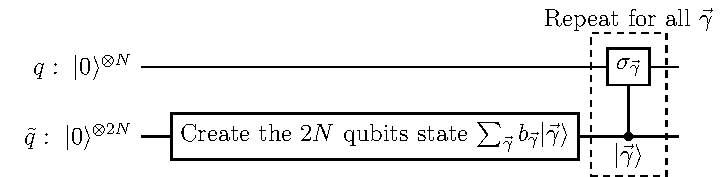
\includegraphics{circuito_general.pdf}
\caption{{\bf Circuit for an $N$-qubit
Pauli channel.}
The circuit creates the state $\sum_{\vec{\gamma}} b_{\vec{\gamma}}|\vec{\gamma}\rangle$ 
on the $2N$ ancilla qubits denoted by $\tilde{q}$.}
\label{Fig1}
\end{figure} % }}}

The first part of the circuit involves the creation of the state
\begin{eqnarray}
\label{eq: state}
\text{Ancilla state =} 
\sum_{\vec{\gamma}} b_{\vec{\gamma}} |\vec{\gamma} \rangle
\end{eqnarray}
on the ancilla qubits, where $b_{\vec{\gamma}}$ are numbers such that $
{|b_{\vec{\gamma}}|}^2 = k_{\vec{\gamma}}$ and
the $2N$-qubit state $|\vec{\gamma}\rangle$ is defined as $|\gamma_1\rangle
\cdots |\gamma_N\rangle$.
When measured in the computational basis, the state given in \eref{eq: state}
collapses to $|\vec{\gamma}\rangle$ with a 
probability ${|b_{\vec{\gamma}}|}^2 = k_{\vec\gamma}$. 
The circuit in \fref{Fig1} uses this fact
to apply $\sigma_{\vec{\gamma}}$ on the main qubits
with a probability $k_{\vec\gamma}$ by using controlled operations 
conditioned on the state of the system being $|\vec{\gamma}\rangle$,
just as the Pauli channel is supposed to do.  

%}}}
\subsection{Simulation for one-qubit Pauli channels} % {{{
\label{subsec: Simulation for one-qubit Pauli channels}

For the particular case of a Pauli channel on one qubit, the circuit that
simulates it can be constructed as in \fref{Fig2},
which is a special case of \fref{Fig1}
but with all details  explicitly shown.
In said figure, the ancilla state
of \eref{eq: state} can be taken to be
$\sqrt{k_{0}} |00\rangle + \sqrt{k_{1}} |01\rangle + \sqrt{k_{2}} 
|10\rangle + \sqrt{k_{3}}|11\rangle$
and it is created on the ancilla qubits with the help of three rotations of angles
defined by the following equations:
\begin{align}
\label{eq:angle}
\cos\left(\dfrac{\theta_0}{2} \right) &= \sqrt{k_{0} + k_{1}},\nonumber \\
\tan\left( \dfrac{\theta_1 + \theta_2}{2} \right) &= \sqrt{k_{1}/k_{0}},  \\
\tan\left( \dfrac{\theta_2 - \theta_1}{2} \right) &= \sqrt{k_{3}/k_{2}}.  \nonumber
\end{align}

\begin{figure} % {{{
\centering
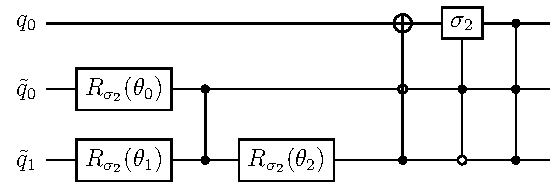
\includegraphics{circuito_unqubit.pdf}
\caption{
{\bf One-qubit Pauli channel circuit.} Circuit for a one-qubit Pauli channel,
which is a particular case of \fref{Fig1}.  Here we have two
ancilla qubits and we use three rotations
of angles given by \eref{eq:angle} to create the Ancilla State of
of \eref{eq: state} for the two ancilla qubits.
}
\label{Fig2} 
\end{figure} % }}}


% We took a sample of one-qubit Pauli channels and
% used the ibmq-lima quantum computer that IBM has available~\cite{Qiskit}
% to simulate them. For each of these channels, we used quantum process
% tomography~\cite{Qiskit, Chuang:1996} to obtain the 
% operator $\xi_I$ corresponding to the implementation of the
% circuit.  Then, we compared this operator with the ideal 
% channel $\xi_T$  we
% wanted to implement.  

We took a sample of one-qubit Pauli channels
and evaluated their implementation on IBM's
ibmq-lima quantum computer~\cite{Qiskit},
as shown in \fref{Fig3}. 
For each of the channels sampled, we used 
quantum process tomography~\cite{Qiskit, Chuang:1996} to obtain the 
operator $\xi_I$ corresponding to the implementation of the
circuit in the quantum computer. 
Then, we compared $\xi_I$ with the theoretical 
operator $\xi_T$ of the Pauli channel we wanted to implement.
To see how close the operators $\xi_I$ and 
$\xi_T$ are, we shall use the
diamond distance~\cite{wildebook}, which is defined by
\begin{equation}
||\xi_I - \xi_T ||_{\diamond}  = \max_{\rho} || (\xi_I \otimes I) \rho - (\xi_T \otimes I) \rho ||_1,
\end{equation}
with $I$ the identity map,
$|| \cdot ||_1$ the trace norm and the maximization
done over all density matrices $\rho$.
The calculation of this norm is done using the semi-definite program from reference \cite{Watrous}.
When the two channels are the same,
the diamond distance has a value of $0$, while in the case that the channels
are completely distinguishable, the distance reaches its maximum value of $2$~\cite{Benenti}.
For the analysis done in \fref{Fig3}, we define a sort of ``diamond fidelity'' as: 
\begin{equation}
f = 1 - \dfrac{1}{2} ||\varepsilon_I - \varepsilon_T ||_{\diamond},
\label{eq:diamond-fid}
\end{equation}
which ranges from $0$, when the channels have a maximum distance, to  $1$,
when they are exactly equal.

\begin{figure} % {{{
\centering
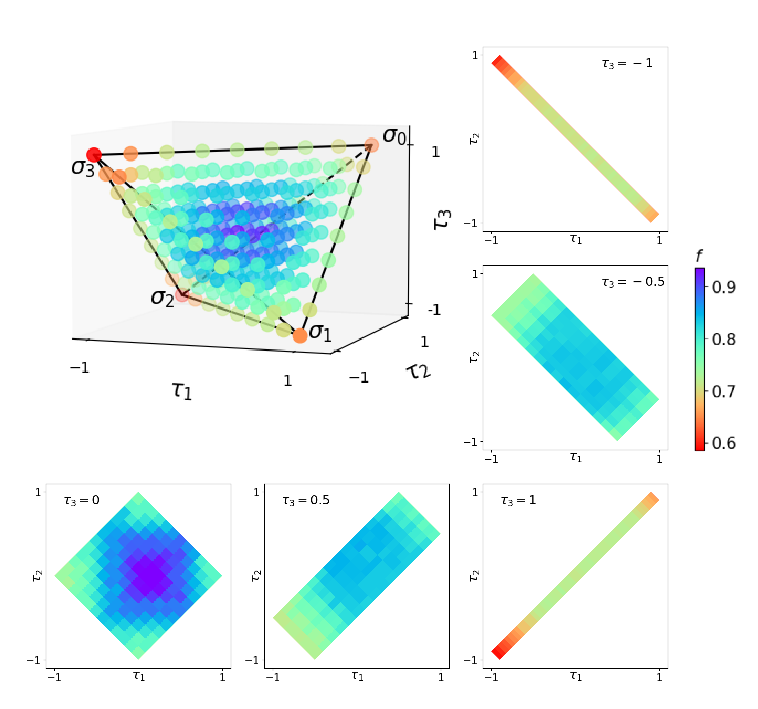
\includegraphics{fig-tetra.pdf}
\caption{{\bf Results of the diamond fidelities as defined in \eref{eq:diamond-fid}
for a sample of Pauli channels in the tetrahedron.}  Notice that channels close
to the center of the tetrahedron have high fidelities, while those close to the
borders do not.  Moreover, we show the results for cuts of the tetrahedron at
different values of $\tau_3$.}
\label{Fig3}
\end{figure} % }}}

Finally, using the representation of Pauli channels in a tetrahedron as in
\eref{eq: conditions-tetrahedron}, we show in \fref{Fig3} the diamond
fidelity defined by \eref{eq:diamond-fid} for the channels analyzed.  We can
see that channels close to the completely depolarizing channel (that is close
to the center of the tetrahedron) have a high $f$, while those close to unitary
channels have much lower $f$. 
% \revnote{So another way to see this is that the simulation through the
% proposed decomposition works only for depolarising channels, and fails
% otherwise. } 
% \tbnote{Contestar en la carta que funciona hasta cierto punto para todos los
% canales propuestos y que se cuantifica qué tan bien funciona o no usando la
% fidelidad}
This is reasonable because quantum computers are
prone to errors that depolarize qubits, which isn't very problematic when
trying to simulate depolarization but it is when simulating unitary processes.
% Moreover, the algorithm of \fref{Fig2} is not optimal for
% unitary channels (that is, the channels corresponding to the vertices of the
% tetrahedron). \revnote{why?} \tbnote{Replantear, decir que cerca de los vertices del tetraedro teneos una fidelidad
% baja segun la imagen, por lo que podemos ver que los unitarios
% tienen una fid baja.} 
% \tbnote{
Moreover, as can be seen in \fref{Fig3}, the algorithm of \fref{Fig2} is not optimal for 
channels in the edges of the tetrahedron, which corresponds to unitary channels. 
% }
These channels could be accomplished more
efficiently by simply applying the corresponding unitary operator directly. 
% \revnote{I wholeheartedly agree with this statement, and I would go so far as
% to claim that this is true in general, even at the center of the tethraedron.}
% \tbnote{Este comentario se conecta con lo del 
% primer comentario, que no sé bien cómo contestar.}
% Nevertheless, due to its general design to accommodate any Pauli channel, the
% algorithm employs numerous quantum gates even in such scenarios. 
In this case we would be trading generality for fidelity. 
% \revnote{but this is a severe disadvantage, that begs the question: what is the advantage?}
% \tbnote{Se podría entonces cambiar la ultima oración del texto por la siguiente para que quede más claro:}
The main advantage of the algorithm is that we can simulate with a unitary 
circuit
% simple, and if we want 
% to 
any Pauli channel, 
% (for example,
% for simulating a Pauli dynamical map as we will see later),
only varying a couple of angles in the circuit.
%  to move between 
% different Pauli channels and not completely reconstruct the circuit. 
In fact, as we will see, sometimes only changing one angle in the circuit will
be enough to simulate many non-unitary dynamical maps of physical interest. 


% {\color{green} This disadvantage comes from the fact
% that the circuit is applicable to any Pauli channel, which that means that sometimes
% it is not the most straightforward algorithm to simulate a Pauli channel.
% However, the main advantages are that the algorithm is simple, and if we want 
% to simulate many Pauli channels (for example,
% for simulating a Pauli dynamical map as we will see later),
% we only have to change a couple of angles in the circuit to move between 
% different Pauli channels and not completely reconstruct the circuit. 
% And as we will see, sometimes only changing
% one angle in the circuit will be enough.}\\
% $\;$\\
% 
% \tbnote{Sección que agregué:}\\
% }}}
\subsection{Simulation of a two-qubit Pauli channel} \label{2qbit-s} % {{{
% {\color{green}
For the general case of a two-qubit Pauli channel,
the circuit of \fref{Fig1} requires two main
qubits and four ancilla qubits.
% , on which it would be necessary to create the state $\sum_{\vec{\gamma}}
% b_{\vec{\gamma}} |\vec{\gamma}\rangle$.
However, the quantum computer which we are using has only 5 qubits.
We could still simulate a two qubit Pauli channel that applies at most $8$ Pauli operations,
instead of 16 which would be the most general case,
using the three ancilla qubits. 
For example, consider the following two-qubit dephasing channel:
\begin{align}
\varepsilon (\rho) = (1-p) \rho + \dfrac{p}{3} (I \otimes \sigma_z) \rho (I \otimes \sigma_z) +  \dfrac{p}{3}(\sigma_z \otimes I) \rho (\sigma_z \otimes I) +  \dfrac{p}{3}(\sigma_z \otimes \sigma_z) \rho (\sigma_z \otimes \sigma_z),
\label{2qbit-c}
\end{align}
where $p \in [0,1]$ is a parameter that defines the channel. 
Since this channel has four Pauli operations, 
only $2$ ancilla qubits will be necessary, and thus it can be implemented
using the circuit of \fref{2qbit}b.

\begin{figure} % {{{
\centering
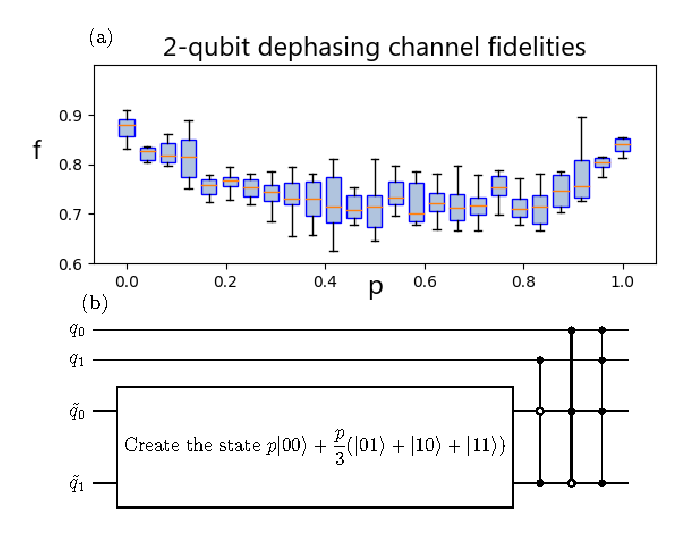
\includegraphics{images/qbit-im.pdf}
\caption{{\bf Circuit for 2-qubit dephasing channel.}  Circuit implementation
for the 2-qubit dephasing channel of \eref{2qbit-c} and fidelity results of its implementation using ibmq-lima.
 The circuit is shown in figure a), where the  state on the two
ancilla qubits can be constructed just as it was done for \fref{Fig2}. 
In figure b) we show the results of fidelities after implementing
this circuit on ibmq-lima for $25$ values of $p$ between $0$ and $1$, 
each of which is simulated $10$ times.
}
\label{2qbit}
\end{figure} % }}}

Just as for the one-qubit Pauli channels, this 
channel was implemented on IBM's ibmq-lima  quantum computer. We obtained the Choi 
matrix by doing quantum process tomography on
the main qubits. Then, we calculated the diamond fidelity for different values of $p$ and
obtained the results shown in \fref{2qbit}a. 
As can be seen in the figure, the fidelity doesn't vary much as we change the value of $p$.
The average fidelity over all values of $p$ is $0.758$ and it is biggest when $p=0$,
corresponding to the identity channel, where it reaches a fidelity of $0.874$.

% }}}
% }}}
\section{One parameter circuits} % {{{
\label{sec: 1PR Circuits}

% {\color{green}
% Finally, we move to the main goal of this article, which is 
% simulating Pauli dynamical maps.
% 
Finally, we consider the simulation of 
Pauli dynamical maps.
% 
This is pretty much already solved, since
just as Pauli channels, Pauli dynamical maps can be implemented using the circuit
of \fref{Fig1}. However, there is one difference: 
the state to be created on the ancilla qubits now 
depends on a parameter $p$, and it is represented by the expression:
\begin{eqnarray}
\label{eq: parametrized state}
\sum_{\vec{\gamma}} b_{\vec{\gamma}}(p) |\vec{\gamma}\rangle.
\end{eqnarray}
Thus, we temporarily shift our focus from Pauli
channels and dynamical maps to the general problem of 
creating a circuit to generate a curve of
states like the one described in \eref{eq: parametrized state}.

In general, producing this curve of states for $N$ qubits will require
many rotations parametrized by $p$,
such as the three rotations used for the ancilla
qubits in \fref{Fig2}.
However, it would be preferable to achieve the same effect using only one parametrized rotation.
This would allow us to interpret said rotation 
as a knob that smoothly traverses the curve of states.
Consequently, we are faced with the question of which curves of states, 
such as the one described in \eref{eq: parametrized state}, 
can be produced using just a single parametrized rotation. 
To clarify this, we provide the following definition 
for a circuit with one parametrized rotation.

\begin{definition}{\textbf{1-Parameter Rotation Circuit:}}
A 1-Parameter Rotation (1PR) circuit is a parametrized quantum
circuit that includes only one gate dependent on a parameter $p$.
Moreover, the parametrized gate is a one-qubit rotation about any axis,
whether controlled or not.
\end{definition}
% \revnote{This definition is vague - given the vagueness of the term "quantum circuit".
%  Here what you are defining is just a unitary operation acting on a N-qubit Hilbert space, that is parameter dependent only locally on one specific qubit.}
%  \tbnote{Agregar lo siguiente a la definición:} 
%  
Therefore, a 1PR circuit implements a unitary operator $U(p)$ on some number $N$ of qubits,
such that $U$ depends on the parameter $p$ only locally on one specific qubit.

Based on this definition, we aim to determine which curves of 
states can be generated using 1PR circuits. 
To accomplish this, we begin by proving that all 1PR circuits have 
the form depicted in \fref{Fig4},
where the parametrized rotation is around $\sigma_3$ and
is applied to the last qubit.

\begin{figure} % {{{
\centering
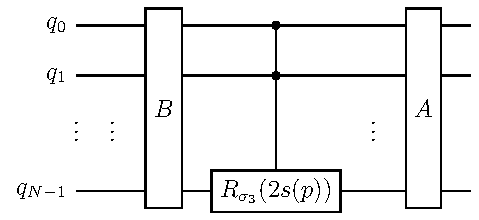
\includegraphics{OPR-circuit.pdf}
\caption{\textbf{General form of a 1PR circuit}.
Any 1PR circuit can be transformed into this form,
where the rotation on the last qubit
can be controlled or not by any of the other qubits.
$A$ and $B$
are $N$-qubit gates that do not depend on the parameter $p$ and
$s= s(p)$ is a function of the parameter.}
\label{Fig4}
\end{figure} % }}}

\begin{theorem}
An $N-$qubit 1PR circuit can always be transformed 
into the form shown in \fref{Fig4}.
\end{theorem}
\textbf{Proof:} 
First, we observe that according to the
definition, a 1PR circuit always consists of an operation $B$ followed 
by the parametrized rotation on a specific qubit and then another operation $A$, 
where $A$ and $B$ are not parametrized.

Next, we note that it is not necessary to consider rotations about an arbitrary axis,
as a rotation about any axis $\hat{n}$ parameterized by $p$
can be transformed into a rotation about $\sigma_3$ without introducing 
gates that depend on $p$. To see this, consider the rotation $R_{\hat{n}}(2s)$, where $2s$ 
is a function of $p$ (the factor of 2 is for convenience later on) 
and $\hat{n} = (n_1,n_2,n_3)$ represents the rotation axis. 
We can express $\hat{n}$ as $(\sin \theta \cos \phi, \sin \theta \sin \phi, \cos \theta)$, 
where $\theta$ and $\phi$ are fixed angles dependent on $\hat{n}$. 
The rotation can then be rewritten as follows:
\begin{eqnarray}
R_{\hat{n}}(2s) = R_{\sigma_3}(\phi) R_{\sigma_2}(\theta) R_{\sigma_3}(2s) R_{\sigma_2}(-\theta) R_{\sigma_3}(-\phi).
\end{eqnarray}
Since the angles $\theta$ and $\phi$ do not depend on the parameter $p$,
any 1PR circuit can be transformed into a circuit where the parametrized
 rotation is around $\sigma_3$ instead of an arbitrary axis. 
Moreover, without loss of generality, we can choose the last qubit as the
target qubit for the rotation, since if it is not, we could use
swap gates to move the rotation
to the first qubit without adding gates
that depend on $p$. 

Therefore, a 1PR circuit can be transformed such
that the rotation is around $\sigma_3$ and is applied to the last qubit 
(possibly controlled by other qubits), 
resulting in the form depicted in \fref{Fig4}. 
$\blacksquare$ \\
$\;$\\

With the aid of this theorem, we can now determine the curves
of states of $N$ qubits that can be generated using a 1PR circuit. 
This result is stated in the following theorem.

\begin{theorem}
\label{theorem2}
Consider a 1PR circuit of $N$ qubits parametrized by $p$
and denote by $U(p)$ the operator it implements on this system. 
Then, for every $j \in \{0, 1, \cdots, 2^N-1\}$, 
we have that:
\begin{align}
U(p)|j\rangle = e^{is(p)} |a^j\rangle + e^{-is(p)} |b^j\rangle + |c^j\rangle
\label{eq:uj}
\end{align}
with $s(p)$ some function of $p$,  $|a^j\rangle ,|b^j\rangle, |c^j\rangle$ orthogonal states 
and $\langle a^j| a^j\rangle + \langle b^j| b^j\rangle + \langle
c^j|c^j \rangle = 1$. Here $|j\rangle$ represents an element of the N-qubit  computational basis.
\end{theorem}
\textbf{Proof:}  
% \revnote{again, this is not a conclusion from theorem 1. This is literally
% Definition 1. Also, use the proper notation here - make A and B operators
% living on an dim N Hilbert state, and R explixitly dependent on s and operating
% on qubit N. Then the matrix representation of the operators is a $2^n \times
% 2^n$ matrix which is applied to the state j.... The explanation in words in not
% sufficient.} \tbnote{Cambié la siguiente oración por el párrafo en verde}
% We can conclude from theorem 1 that $U=ARB$,
% where $A$ and $B$ are unitary matrices and $R$ is a $\sigma_3$ rotation of angle $2s$
% applied to the last qubit and controlled by some of the other ones. 
% {\color{green} 
As before, from the definition of a 1PR circuit, we know that $U(p)$ can be
decomposed as $ARB$, where $A,B$ are unitary operators acting on the $N$-qubit
system and $R$ is a rotation applied to one qubit.  From theorem 1, we conclude
that $R$ can be taken in general as a $\sigma_3$ rotation of angle $2s(p)$
applied to the last qubit and controlled by some of the other ones.  To prove
this theorem, we will apply $U(p)$ to $|j\rangle$ by first applying $B$, then
$R_{\sigma_3}(2s(p))$ and finally $A$, with the goal of getting to
\eref{eq:uj}. 
% }

First, applying $B$ to $|j\rangle$ results in $B|j\rangle = B_{0,j} |0\rangle + B_{1,j} |1 \rangle + \cdots + B_{2^n-1,j}|2^n-1\rangle$,
with $B_{i,j}$ the entries of matrix $B$.
This can be rewritten by separating the last qubit from the other $N-1$:
\begin{equation}
B|j\rangle = \sum_{k=0}^{2^{N-1}-1} \left( B_{2k,j} |k\rangle|0\rangle  + B_{2k+1,j} |k \rangle |1\rangle  \right).
\end{equation}
After the operator $B$, the circuit applies the  controlled rotation $R_{\sigma_3}(2s(p))$.
To simplify the analysis, we separate the states of
the first $N-1$ qubits into those that fulfill the control conditions of the rotation
(which we denote as the set $\mathcal{C}$)
and those that do not, and write it as
\begin{align}
B|j\rangle = 
   \sum_{k \in \mathcal{C}} \left( B_{2k,j} |k\rangle|0\rangle 
                                     + B_{2k+1,j} |k \rangle |1\rangle  \right) 
   + \sum_{k \not\in \mathcal{C}} \left( B_{2k,j} |k\rangle|0\rangle  
                                      + B_{2k+1,j} |k \rangle |1\rangle  \right).
\end{align}

Then, the rotation $R$ will only affect the states on the first sum (since they fulfill the control conditions)
and not the others. Therefore,  
using that a $R_{\sigma_3}(2s(p))$ rotation acts by adding a phase $e^{-is(p)}$ to $|0\rangle$
and a phase $e^{is(p)}$ to $|1\rangle$, we have that,
% \begin{small}
% \begin{eqnarray}
% &e^{-is} \sum_{k \in \mathcal{C}} B_{2k,j} |k\rangle |0\rangle + e^{is} \sum_{k \in \mathcal{C}} B_{2k+1,j} |k\rangle |1 \rangle 
% + \sum_{k \not\in \mathcal{C}} \left( B_{2k,j} |k\rangle |0\rangle + B_{2k+1} |k\rangle |j \rangle \right)\\
% & \qquad = e^{-is} \vec{b'}_j + e^{is} \vec{a'}_j + \vec{c'}_j,
% \end{eqnarray}
% \end{small}
% test
\begin{small}
\begin{align}
R_{\sigma_3}(2s(p))B|j\rangle& = e^{-is(p)} \sum_{k \in \mathcal{C}} B_{2k,j} |k\rangle |0\rangle + e^{is(p)} \sum_{k \in \mathcal{C}} B_{2k+1,j} |k\rangle |1\rangle 
+ \sum_{k \not\in \mathcal{C}} \left( B_{2k,j} |k\rangle|0\rangle  + B_{2k+1,j} |k \rangle |1\rangle  \right) \nonumber \\
& = e^{-is(p)} |\tilde{b}^{j}\rangle + e^{is(p)} |\tilde{a}^j\rangle + |\tilde{c}^j\rangle,
\end{align}
\end{small}
where we defined
\begin{align*}
|\tilde{a}^j \rangle &= \sum_{k \in \mathcal{C}} B_{2k,j}|k\rangle|1\rangle,\\
|\tilde{b}^j\rangle &= \sum_{k \in \mathcal{C}} B_{2k+1,j} |k\rangle |0 \rangle,\\
|\tilde{c}^j\rangle &= \sum_{k \not\in \mathcal{C}}\left( B_{2k,j} |k\rangle|0\rangle+ B_{2k+1,j} |k \rangle |1\rangle  \right).
\end{align*}
These states are clearly orthogonal because they are each linear combinations of different 
orthogonal states of the computational basis. 
Moreover, they satisfy  $\langle a^j| a^j\rangle + \langle b^j| b^j\rangle + \langle c^j| c^j\rangle = 1$ because this quantity is the squared norm of the $j$th column of $B$, 
which is unitary. 


Finally, after having applied the rotation, the circuit applies gate $A$, 
so that the result is given by:
% \begin{eqnarray*}
\begin{align}
U|j\rangle &= AR_{\sigma_3}(2s(p)) B|j\rangle \nonumber \\
           &= e^{-is(p)} A |\tilde{a}^j\rangle + e^{is(p)} A |\tilde{b}^j\rangle 
              + A |\tilde{c}^j\rangle \nonumber \\
           &= e^{-is(p)} |a^j\rangle + e^{is(p)} |b^j\rangle + |c^j\rangle,
\end{align}
% \end{eqnarray*}
where $|a^j\rangle = A |\tilde{a}^j\rangle, |b^j\rangle = A |\tilde{b}^j\rangle, |c^j\rangle = A |\tilde{c}^j\rangle$ are still orthogonal
states that satisfy $\langle a| a\rangle + \langle b| b\rangle + \langle c| c\rangle = 1$ because $A$ is unitary. $\blacksquare$  \\
 $\;$ \\

This theorem implies that when starting from the state $|0\rangle$ 
or any other initial state, the only possible curves of states that can be 
created using a 1PR circuit are of the following form:
\begin{equation}
|\eta(p)\rangle = |c\rangle + e^{is(p)}|a\rangle + e^{-is(p)} |b\rangle,
\label{eq:curve-states}
\end{equation}
with conditions defined by the equations: 
\begin{equation}
\langle a| a\rangle + \langle b| b\rangle + \langle c| c\rangle = 1,  \quad
\langle a |b\rangle =
\langle a |c\rangle =
\langle b |c\rangle = 0.
\label{eq:conditions-vecs}
\end{equation}

Moreover, it is possible to construct a 1PR circuit to generate any given curve of 
states described by \eref{eq:curve-states}. 
One approach to achieve this is by utilizing the circuit 
depicted in \fref{Fig4}, 
with the parametrized rotation $R$ applied to the last qubit controlled by all the 
other qubits. There is some freedom when choosing
the operators $A$ and $B$, we only need
to make sure that:
\begin{align}
&B|0\rangle = \sqrt{\langle a | a \rangle} |2^{N}-1 \rangle + \sqrt{\langle b | b \rangle} |2^{N}-2\rangle + \sqrt{\langle c |c \rangle} |2^N-3\rangle, \nonumber \\
&A|2^N-1 \rangle = \frac{1}{\sqrt{\langle a | a \rangle}} |a\rangle,\; A|2^{N}-2\rangle = \frac{1}{\sqrt{\langle b | b \rangle}}|b\rangle, \; A|2^{N}-3\rangle = \frac{1}{\sqrt{\langle c | c \rangle}}|c\rangle.
\label{eq:BA}
\end{align}
The remaining part of the operators $A$ and $B$ can be chosen
in any arbitrary manner as long as they are unitary. 
Examples of these matrices are shown for particular dynamical maps in the next section.
%Then, by following the calculations of applying 
%$A R_{\sigma_3}(2s(p)) B$ to $|0\rangle$,
%it can be shown that the curve of states created is that described in \eref{eq:curve-states}.

To see that $A R_{\sigma_3}(s(p)) B |0\rangle$ in fact creates
the curve of states described in \eref{eq:curve-states}, we can rewrite the expression of $B|0\rangle$ by 
separating the first $N-1$ qubits from the last one:
$$B|0\rangle = \sqrt{\langle a | a \rangle} |2^{N-1}-1\rangle |1\rangle + \sqrt{\langle b | b \rangle} |2^{N-1}-1\rangle |0\rangle + \sqrt{\langle c | c \rangle} |2^{N-1}-2\rangle |1\rangle.$$
Since the parametrized rotation $R_{\sigma_3}(2s(p))$ is controlled by all the first $N-1$ qubits, it only applies to the first two terms of $B|0\rangle$. As a result, we obtain: 

$$
R_{\sigma_3}(2s(p))B|0\rangle =\sqrt{\langle a | a \rangle} e^{is(p)} |2^{N-1}-1\rangle |1\rangle + \sqrt{\langle b | b \rangle} e^{-is(p)} |2^{N-1}-1\rangle |0\rangle + \sqrt{\langle c | c \rangle} |2^{N-1}-2\rangle |1\rangle.
$$

Finally, applying the  operator $A$ to this state yields: 
\begin{align*}
AR_{\sigma_3}(2s(p))B = |c\rangle + e^{is(p)} |a\rangle + e^{-is(p)} |b\rangle.
\end{align*}
With this, we prove that any curve of states as that in \eref{eq:curve-states} 
can be constructed by the circuit in  \fref{Fig4} with the parametrized rotation 
controlled by all the other qubits 
by correctly choosing matrices $A$ and $B$.

 
% }}}
\section{1PR circuit for a Pauli map} % {{{
\label{sec: 1PR circuit for a Pauli map}

We can now use the previous results to conclude directly which Pauli dynamical maps
can be implemented with a 1PR circuit.
For this, the curve of states of \eref{eq: parametrized state} 
has to be constructed with only one parametrized rotation,
so it has to satisfy the conditions of theorem \ref{theorem2}.
Therefore, this implies that the map
\begin{eqnarray}
\varepsilon_p(\rho) = \sum_{\vec{\gamma}} k_{\vec{\gamma}}(p) \sigma_{\vec{\gamma}} \rho \sigma_{\vec{\gamma}},
\end{eqnarray}
can be implemented  if there are numbers $\beta_{\vec{\gamma}}(p)$ such that $|\beta_{\vec{\gamma}}(p)|^2 = k_{\vec{\gamma}}(p)$ and
\begin{eqnarray}
\label{eq:vec}
\sum_{\vec{\gamma}} \beta_{\vec{\gamma}}(p) |\vec{\gamma}\rangle = |c\rangle +  e^{is(p)} |a\rangle + e^{-is(p)}|b\rangle,
\end{eqnarray}
where $|a\rangle,|b\rangle,|c\rangle$ fulfill
the conditions of \eref{eq:conditions-vecs}.

For the particular case of one qubit, we can show some examples of Pauli
dynamical maps implementable with a 1PR circuit, which are plotted in
\fref{Fig5}. 
The examples we show include some of the most common maps: the bit flip, phase flip, bit-phase flip and depolarizing.
However, we also include the parabolic dynamical map,
defined in \eref{eq:parab} and shown in \fref{Fig5}.
This map traces a parabola inside the tetrahedron connecting two of its vertices
and it describes a frontier in the tetrahedron between Pauli channels
that are reachable by Lindbladian dynamics and those that are not~\cite{Davalos}.

\begin{figure} % {{{
\centering
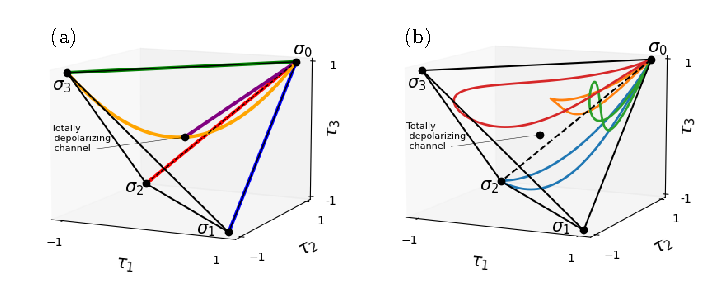
\includegraphics{fig-curves.pdf}
\caption{{\bf Some Pauli dynamical maps that can be implemented with a 1PR circuit.}
The curves painted in these tetrahedrons
represent Pauli dynamical maps that can be implemented with 1PR circuits.
(a) shows the dynamical maps mentioned in the main 
text, which are: depolarizing (purple), bit flip (blue),
phase flip (green), bit-phase flip (red)
and parabolic (orange).
(b) shows dynamical maps selected at random that can be implemented with 1PR 
circuits.}
\label{Fig5}
\end{figure} % }}}


\begin{itemize}
\item \textbf{Depolarizing:} This dynamical map is given by
\begin{align}
\varepsilon_p(\rho) = (1-3p/4) \rho + (p/4) \sigma_1 \rho \sigma_1 + (p/4) \sigma_2 \rho \sigma_2 + (p/4) \sigma_3 \rho \sigma_3,
\label{eq:depo}
\end{align}
with $p \in [0,1]$. 
Therefore, the curve of states $|\beta(p)\rangle$ needed on the ancilla
qubits is such that ${|\beta_0(p)|}^2= (1-3p/4)$, ${|\beta_1(p)|}^2 =
{|\beta_2(p)|}^2 = {|\beta_3(p)|}^2 = p/4$.  Then, taking the $\beta_j$ to be
real, the curve of states can be 
\begin{align*}
|\beta(p) \rangle = \sqrt{1-3p/4} |0\rangle + \sqrt{p/4} |1\rangle + \sqrt{p/4} |2 \rangle  + \sqrt{p/4} |3\rangle.
\end{align*}
This state can be rewritten as:
\begin{align*}
|\beta(p)\rangle =& \; e^{is} \left( \dfrac{1}{2} |0\rangle - \dfrac{i}{2\sqrt{3}} |1\rangle 
      - \dfrac{i}{2\sqrt{3}} |2 \rangle - \dfrac{i}{2\sqrt{3}} |3\rangle \right) \\
& + e^{-is} \left( \dfrac{1}{2} |0\rangle + \dfrac{i}{2\sqrt{3}} |1\rangle 
      + \dfrac{i}{2\sqrt{3}} |2\rangle + \dfrac{i}{2\sqrt{3}} |3 \rangle \right) \\
\equiv &\; e^{is} |a\rangle + e^{-is} |b\rangle
\end{align*}
with $\sin s = \sqrt{3p/4}$.
We can see that this curve satisfies the conditions of \eref{eq:conditions-vecs}, meaning that it can be created with a 
1PR circuit.
Explicitly, following the discussion after theorem \ref{theorem2},
we know that this curve of states can be constructed by 
the circuit of \fref{FigS2q}.

\begin{figure} % {{{
\centering
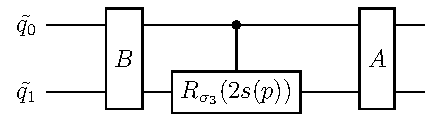
\includegraphics{images/estado-2-qbits.pdf}
\caption{
{\bf 1PR Circuit for one qubit curve of states.} This is a 1PR circuit for creating a curve of states that satisfies
the conditions of theorem \ref{theorem2}. 
given the curve of states, operations $A$ and $B$ can be defined as in \eref{eq:BA}.
}
\label{FigS2q} 
\end{figure} % }}}

The circuit requires defining $A$ and $B$ as in  \eref{eq:BA}, and for the particular
vectors $|a\rangle, |b\rangle, |c \rangle$ of this dynamical map, we have that
\begin{align*}
A = \begin{pmatrix}
0 & 0 & 1/\sqrt{2} & 1/\sqrt{2} \\
1/\sqrt{6} & -1/\sqrt{2} & i /\sqrt{6} & -i /\sqrt{6} \\
1/\sqrt{6}  & 1/\sqrt{2} & i/\sqrt{6} & -i/\sqrt{6} \\
-\sqrt{2/3} & 0 & i/\sqrt{6} & -i/\sqrt{6}
\end{pmatrix} , \; B = \begin{pmatrix}
0 & 0 & 0& 1 \\
0 & 0 & 1 & 0 \\
1/\sqrt{2} & -1/\sqrt{2} & 0 & 0 \\
1/\sqrt{2} & 1/\sqrt{2} & 0 & 0 
\end{pmatrix},
\end{align*}
where, as mentioned before, the first column of $A$ and the
last three of $B$ can be chosen arbitrarily as long as the resultant matrices are unitary. 
We ran this circuit in IBM's quantum computer ibmq-lima for $25$ different values of $p$ between $0$ and $1$,
with $20$ repetitions for each value of $p$.
The diamond fidelity was calculated in each case and is shown in \fref{fid}.

\item \textbf{Parabolic dynamical map:} We define the parabolic dynamical map as:
\begin{eqnarray}
\epsilon(\rho) =  {(1-p)}^2  \rho + (p-p^2) \sigma_1 \rho \sigma_1 + (p-p^2) \sigma_2 \rho \sigma_2 + p^2 \sigma_3 \rho \sigma_3,
\label{eq:parab}
\end{eqnarray}
with $p \in [0,1]$. 
If we take the $\beta_j$ to be real,
the curve of states needed on the ancilla qubits can be:
\begin{eqnarray}
|\beta(p)\rangle =  (1-p) |0\rangle + \sqrt{p-p^2} |1\rangle +  \sqrt{p-p^2} |2\rangle + p |3\rangle.
\end{eqnarray}
This can be rewritten as
\begin{align*}
|\beta(p)\rangle =&\; \left( \dfrac{1}{2}|0\rangle + \dfrac{1}{2} |3\rangle \right) + e^{is} \left( \dfrac{i}{4}|0\rangle + \dfrac{1}{4} |1\rangle + \dfrac{1}{4} |2\rangle - \dfrac{i}{4} |3\rangle \right) \\
& + e^{-is}  \left( \dfrac{-i}{4} |0\rangle + \dfrac{1}{4} |1\rangle + \dfrac{1}{4} |2\rangle + \dfrac{i}{4} |3\rangle \right) \\
\equiv & \; |c\rangle + e^{is} |a\rangle + e^{-is} |b\rangle,
\end{align*}
with $\sin s = 2p-1$, so that
this curve fulfills the conditions of  \eref{eq:conditions-vecs}.
This  means that it can be created with the
1PR circuit of figure \fref{FigS2q}. In this
case, matrices $A$ and $B$ can be taken to be:
\begin{align*}
A = \begin{pmatrix}
0 & 1/\sqrt{2} & -i/2 & i/2 \\
-1/\sqrt{2} & 0 & 1/2 & 1/2 \\
1/\sqrt{2} & 0 & 1/2 & 1/2 \\
0 & 1/\sqrt{2} & i/2 & -i/2
\end{pmatrix},
B = \begin{pmatrix}
0 & 1 &0 &0 \\
1/\sqrt{2} & 0 & 0 &-1/\sqrt{2} \\
1/2 & 0 & 1/\sqrt{2} & 1/2 \\
1/2 & 0 & - 1/\sqrt{2} & 1/2
\end{pmatrix},
\end{align*}
where again, the first column of $A$ and the last three of $B$ can be chosen arbitrarily. 
As before, we ran this circuit for $25$ values of $p$ between $0$ and $1$, with $20$ repetitions for each,
obtaining as a result the fidelities shown in \fref{fid}.




\item \textbf{Bit flip map:} 
This dynamical map is defined as
\begin{align*}
\varepsilon_p(\rho) = (1-p)\rho + p\sigma_1 \rho \sigma_1,
\end{align*}
for $p \in [0,1]$. 
In particular, if we take the $\beta_j$ to be real,
we need to create the curve of states:
\begin{align*}
|\beta(p)\rangle = \sqrt{1-p} |0\rangle +\sqrt{p} |1\rangle.
\end{align*}
This can be rewritten as
\begin{align*}
|\beta(p) \rangle = e^{is}  \left(\frac{1}{2} |0\rangle - \dfrac{i}{2} |1\rangle \right) + e^{-is} \left( \frac{1}{2} |0\rangle + \frac{i}{2} |1\rangle \right),
\end{align*}
with $\sin s= \sqrt{p}$.
Therefore, we can see that the curve satisfies the conditions of  \eref{eq:conditions-vecs} 
and it can be created with a 1PR circuit.
Matrices $A$ and $B$ can be obtained as for the other
dynamical maps and we ran the resulting circuit in ibmq-lima with the same
specifications as for the other examples,
with the results are shown in \fref{fid}.
%Note that in this case we actually only need one ancilla qubit
%since the state $|\beta(p)\rangle$ is only two dimensional.

The exact same thing can be done
for the phase flip and bit phase flip dynamical maps by
changing $\sigma_1$ to
$\sigma_3$ and $\sigma_2$ respectively.
For example, the bit phase flip map was implemented in \cite{Andrea, Andrea_4qb} 
using an optical arrangement, and  it was indeed done 
by varying only one angle that depends on the parameter $p$ (the angle of a
half waveplate). 
% \revnote{there is literally one parameter in one qubit, of
% course it depends on one parameter...
%  how can this be a result?}
% \tbnote{Aquí la verdad no entiendo del todo qué intenta decir.
% El resultado es que en ese paper sólo hubo que variar un parámetro
% para hacer el bit phase flip, que coincde con lo que nosotros 
% probamos sobre qué canales se pueden hacer con una rotación parametrizada (pues bit phase flip es uno de esos). }


\end{itemize}

{\color{green}
\begin{figure} % {{{
\centering
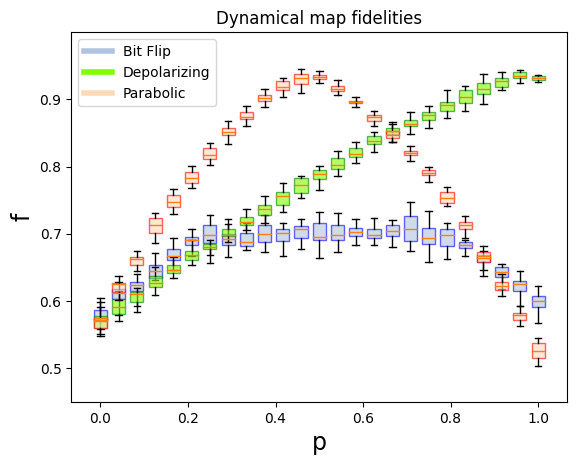
\includegraphics[width=0.60\textwidth]{images/dynamic-fidelitites.png}
\caption{
{\bf Fidelities for dynamical maps.} Results of the fidelities obtained when simulating the three dynamical maps considered (depolarizing, parabolic and bit flip). 
The implementation was done on IBM's ibmq-lima quantum computer.
Furthermore, we can see that the fidelities are comparable to those of \fref{Fig3}, so that using the 1PR circuit
doesn't considerably affect fidelity.}
\label{fid} 
\end{figure} % }}}
}

From the results of \fref{fid}, we can see that just as in figure 
\fref{Fig3}, fidelities are high for points close to the depolarizing channel 
($p=1$ for depolarizing map, $p=1/2$ for parabolic map) and lower for points close
to unitary channels ($p=0$ for all maps and $p=1$ for parabolic and bit flip).
Furthermore, we can see that the actual values of the fidelities are comparable
to those of \fref{Fig3}, which means that
using the 1PR circuit as opposed to 
implementing each channel with \fref{Fig2}
does not considerably affect fidelity.

Furthermore, we can construct other examples of 
Pauli dynamical maps such that they
can be implemented with a 1PR circuit.
To do it, we only need to choose the three states $|a\rangle$, $|b\rangle$, $|c\rangle$
that satisfy the conditions of  \eref{eq:conditions-vecs}.
For example, this can be done systematically for the case of curves of states of two qubits
(that is, for Pauli dynamical maps of one qubit)
with the following procedure:
\begin{itemize}
\item[1.] We first choose the norms $|a|$, $|b|$, $|c|$
such that $\langle a| a\rangle + \langle b| b\rangle + \langle c| c\rangle = 1$. 
This can be done by selecting two angles
$\mu \in [0, \pi/2]$, $\nu \in [0,\pi/2]$ and defining:
\begin{align*}
|a| = \sin \nu \cos \mu, \; |b| = \sin \nu \sin \mu , \; |c| = \cos \nu.
\end{align*}
\item[2.] We define $|a'\rangle = |a| |0\rangle$, $|b'\rangle = |b| |1\rangle$, $|c'\rangle = |c| |2\rangle$.
\item[3.] 
Finally, we choose a unitary matrix $V$ with the condition that its first
row is equal to $e^{i\theta} (|a|,|b|,|c|,0)$
with $\theta$ a uniform random phase.
That way, we can define $|a\rangle = V |a'\rangle$, $|b\rangle = V |b'\rangle$, $|c\rangle = V |c'\rangle$
and since $V$ is unitary, these unprimed vectors will fulfill the conditions of
\eref{eq:conditions-vecs}.
Furthermore, the form of the first row ensures that the dynamical map begins at the identity,
since it implies that when $s=0$, the 
state created in \eref{eq:vec}
is
$|a\rangle + |b\rangle + |c\rangle = e^{i \theta} |0\rangle$,
which  corresponds with applying the identity channel.

Such a matrix $V$ can be randomly constructed by first finding three vectors 
$\vec{w}_1 , \vec{w}_2, \vec{w}_3$ orthogonal to
the first row using the Gram-Schmidt process.  Then selecting random complex
numbers $r_1, r_2, r_3$ such that $|r_1|^2 + |r_2|^2 + |r_3|^2 = 1$ and defining
the second row of $V$ to be $r_1 \vec{w}_1 + r_2 \vec{w}_2 + r_3 \vec{w}_3$.
Once the first two rows are chosen, use Gram-Schmidt to find two vectors
$\vec{v}_1, \vec{v}_2$ orthogonal to 
them and similarly define the third row as $q_1 \vec{v}_1+ q_2 \vec{v}_2$
with $|q_1|^2 + |q_2|^2$ and $q_1,q_2$
selected at random. 
Finally, there is only one choice for the fourth row so that it is 
orthonormal to the first three
and a random phase can be given to it.
\end{itemize}

Following this procedure for random
angles and unitary matrices $V$, 
we plot four Pauli dynamical maps  selected at random
that can be implemented with a 1PR circuit in \fref{Fig5}. 
% \revnote{This is
% interesting, instead of giving only some random examples, I would actually
% explore more in details the zoology of this class of dynamical maps - if lucky,
% you would find class of interesting problems that can be simulated effectively
% in an experimental setup by just accessing one parameter (as the authors say,
% just with one set of waveplates, for example), }
% \tbnote{Los mapas que ya mencionamos más a profundidad (depolarizing, phase damping, etc.) son esos ejemplos creo yo.
% Pues son ejemplos de mapas útiles o conocidos (por lo menos el depolarizing y los bit flip, phase flip, bit phase flip) y que
% probamos que se pueden hacer con una rotación parametrizada.}

% }}}
\section{Conclusion} % {{{

% \revnote{I feel that there needs to be a treatment of what happens, at least qualitatively at higher than two dimension, as one of the selling point is the generality of the formalism for N qubit. I expect, however, that the higher the dimension, the less rich is the space that can be parametrised by only one parameter, so.. what is the applicability of the theorem for higher dimensions?}
% 
% \tbnote{Añadí el párrafo en verde hablando de eso.}
% 
In this work, we found a quantum algorithm for 
simulating Pauli channels in $N$-qubit systems and
generalized it to Pauli dynamical maps
by using parametrized quantum circuits.
%  \revnote{imprecise} \tbnote{No sé exactamente qué es imprecise.}.
Furthermore, we implemented single-qubit Pauli channels
on one of IBM's quantum computers
and obtained their fidelities. 

Then, when working with Pauli dynamical maps,
we searched for a way of minimizing the amount of 
parametric operations in the circuit 
by requiring that only one single-qubit rotation depends on the parameter. 
% \revnote{This reasoning I miss, simplifying for achieving what goal? } 
% \tbnote{Le di una reescritura a esa frase.}
In theorem \ref{theorem2} we found the general mathematical conditions for 
this, applicable to any parametrized circuit.
Given this condition, we considered the space of Pauli maps that are
possible to parametrize with one parameter, and gave some explicit examples for
a system of one qubit.  As the number of qubits gets bigger, the degrees of
freedom for choosing a Pauli dynamical map also gets bigger, so we would expect
that the space of maps that can be done with only one parameter
becomes a relatively smaller part of the whole space of Pauli dynamical maps.
However, some paradigmatic maps as the dephasing one we studied for 2 qubits will still be possible to do with a 1PR circuit (for this
case, this can be seen by noticing that said dephasing channel
has the same form as the depolarizing channel for one qubit,
which we proved to be possible to implement with a 1PR circuit).

In conclusion, this work presents yet another example of the current
exploration into simulating open quantum
systems in quantum computers,
and we observe the effect that the error of a quantum computer have
on these simulations, quantified by the fidelity. 
% \revnote{There is no quantification of this, it´s not even the focus of the paper} \tbnote{ya cambié la oración}
On the other hand, the result
of theorem \ref{theorem2}
shows what can be done with the condition of using only one
parametrized rotation and
can be applied to any quantum algorithm that requires parametrized circuits,
such as those used for quantum machine learning~\cite{Benedetti}.

% }}}
%\section{Supporting information} % {{{
%
%
%% Include only the SI item label in the paragraph heading. Use the \nameref{label} command to cite SI items in the text.
%\paragraph*{S1 Code.}
% \label{S1_code}
% {\bf Simulation of Pauli Channels.} Python code for the simulation of Pauli channels on IBM's quantum computers.
%% 
% \paragraph*{S2 Fig.}
% \label{S2_Fig}
% {\bf Lorem ipsum.} Maecenas convallis mauris sit amet sem ultrices gravida. Etiam eget sapien nibh. Sed ac ipsum eget enim egestas ullamcorper nec euismod ligula. Curabitur fringilla pulvinar lectus consectetur pellentesque.
% 
% \paragraph*{S1 File.}
% \label{S1_File}
% {\bf Lorem ipsum.}  Maecenas convallis mauris sit amet sem ultrices gravida. Etiam eget sapien nibh. Sed ac ipsum eget enim egestas ullamcorper nec euismod ligula. Curabitur fringilla pulvinar lectus consectetur pellentesque.
% 
% \paragraph*{S1 Video.}
% \label{S1_Video}
% {\bf Lorem ipsum.}  Maecenas convallis mauris sit amet sem ultrices gravida. Etiam eget sapien nibh. Sed ac ipsum eget enim egestas ullamcorper nec euismod ligula. Curabitur fringilla pulvinar lectus consectetur pellentesque.
% 
% \paragraph*{S1 Appendix.}
% \label{S1_Appendix}
% {\bf Lorem ipsum.} Maecenas convallis mauris sit amet sem ultrices gravida. Etiam eget sapien nibh. Sed ac ipsum eget enim egestas ullamcorper nec euismod ligula. Curabitur fringilla pulvinar lectus consectetur pellentesque.
% 
% \paragraph*{S1 Table.}
% \label{S1_Table}
% {\bf Lorem ipsum.} Maecenas convallis mauris sit amet sem ultrices gravida. Etiam eget sapien nibh. Sed ac ipsum eget enim egestas ullamcorper nec euismod ligula. Curabitur fringilla pulvinar lectus consectetur pellentesque.
% }}}
%
%\section{Acknowledgments} % {{{
%Support by projects CONACyT 285754, and UNAM-PAPIIT IG101421 is acknowledged. 






% Either type in your references using
% \begin{thebibliography}{}
% \bibitem{}
% Text
% \end{thebibliography}
%
% or
%
% Compile your BiBTeX database using our plos2015.bst
% style file and paste the contents of your .bbl file
% here. See http://journals.plos.org/plosone/s/latex for 
% step-by-step instructions.
% }}}
\bibliography{Bibliography}
\appendix
\end{document}
